\documentclass[a4paper,11pt]{article}
%
% document setup, package import, etc.
%
%
% packages and settings for the worksheet files
%
\usepackage[bf,small]{titlesec}
\usepackage{graphicx}
\usepackage{amsfonts,amssymb,amsmath,fancyhdr}
%\usepackage{import} % needed for subimport
\usepackage{url}
\usepackage{paralist} % needed for compactenum
\usepackage{verbatim} % needed for varbatimiinput
\usepackage{shortlst}
\usepackage{siunitx}
%
%  page layout
%
\setlength{\textwidth}{175mm}
\setlength{\textheight}{240mm}
\setlength{\voffset}{-20mm}
\setlength{\hoffset}{-23mm}
\setlength{\parskip}{0pt}
\setlength{\parindent}{0pt}
\setlength{\footskip}{40pt}
\renewcommand{\baselinestretch}{1.2} \small\normalsize
%
%  Header/footer
%
\fancyhf{} % Clear all fields
\renewcommand{\headrulewidth}{0pt}
\renewcommand{\footrulewidth}{0pt}
\fancyfoot[L]{\footnotesize EMAT20920 2020-21}
\fancyfoot[C]{\footnotesize \thepage}
\fancyfoot[R]{\footnotesize COURSEWORK ASSESSMENT}
%
% Change list-making
%
\renewcommand{\theenumi}{\alph{enumi}}
\def\labelenumi{(\theenumi)}
\renewcommand{\theenumii}{\roman{enumii}}
\def\labelenumii{(\theenumii)}
%
% Change section headers
%
\titlelabel{Question \thetitle:\quad}
%
% First page header
%
\newcommand{\solutionsheader}[2]{
    \pagestyle{fancy}
    \begin{center}
      {\large Department of Engineering Mathematics}\\[3ex]
      \textbf{EMAT20920: Numerical Methods in MATLAB}\\[3ex]
      \textbf{#1}\\
      \textbf{#2}
    \end{center}}
%
% For formatting matlab code with listings
%
\usepackage{listings}
\usepackage{color}
\usepackage{textcomp}
\definecolor{listinggray}{gray}{0.9}
\definecolor{lbcolor}{rgb}{0.9,0.9,0.9}
\lstset{
    backgroundcolor=\color{lbcolor},
    numbers=none,
    numberstyle=\tiny,
    tabsize=4,
    rulecolor=,
    language=matlab,
    basicstyle=\scriptsize\ttfamily,
    upquote=true,
    aboveskip={1.5\baselineskip},
    columns=flexible,
    showstringspaces=false,
    extendedchars=true,
    breaklines=true,
    prebreak = \raisebox{0ex}[0ex][0ex]{\ensuremath{\hookleftarrow}},
    %frame=single,
    showtabs=false,
    showspaces=false,
    showstringspaces=false,
    identifierstyle=\ttfamily,
    keywordstyle=\color[rgb]{0,0,1},
    commentstyle=\color[rgb]{0.133,0.545,0.133},
    stringstyle=\color[rgb]{0.627,0.126,0.941},
    aboveskip=0pt,
    belowskip=2pt,
}
%
% shortcut commands
%
\newcommand{\matcmd}[1]{\colorbox{lbcolor}{\lstinline{#1}}}
\newcommand{\matlab}[1]{\texttt{#1}}
\renewcommand{\vec}[1]{\boldsymbol{#1}}
\newcommand{\order}{\mathcal{O}}

\newenvironment{listcomment}[1][1]{\framed\adjustwidth{-\dimexpr 
#1\leftmargin + \fontdimen2\font}{}}{\endadjustwidth\endframed}

\usepackage[toc,title]{appendix}
\usepackage{caption}

\usepackage{hyperref}

\begin{document}

\solutionsheader{COURSEWORK ASSESSMENT}{Jake Bowhay (UP19056)}

\tableofcontents

\hfill \break

All figures in this report have been saved using \verb*|saveFigPDF| function 
as it automatically resizes the paper to the correct size.
\lstinputlisting{../src/saveFigPDF.m}

\section{Root-finding}
\begin{enumerate}
	\item To find how many solutions each equation has in the given domain I 
	will rearrange all the equations to be equal to zero and then looks for 
	the zeros of the rearranged equations. As a corollary to the intermediate 
	value theorem, if a function is continuous and changes sign in a bracket 
	then that bracket must contain a zero. So I will plot each of the 
	rearranged equation and I look for appropriate brackets. I will use the 
	\verb*|pltFunc| function to plot the functions as it removes values 
	outside a defined limit which prevents MATLAB plotting discontinuous 
	functions as continuous. The limits can then be changed using the 
	property explorer to give a more useful plot.
	\lstinputlisting{../src/q1/pltFunc.m}
	\begin{enumerate}
		\item Rearranging $x^{4} = e^{-x} \cos(x)$ gives $f(x) = x^{4} - 
		e^{-x} \cos(x)$.
		\lstinputlisting{../src/q1/Q1a_i.m}
		\NoIndent{
			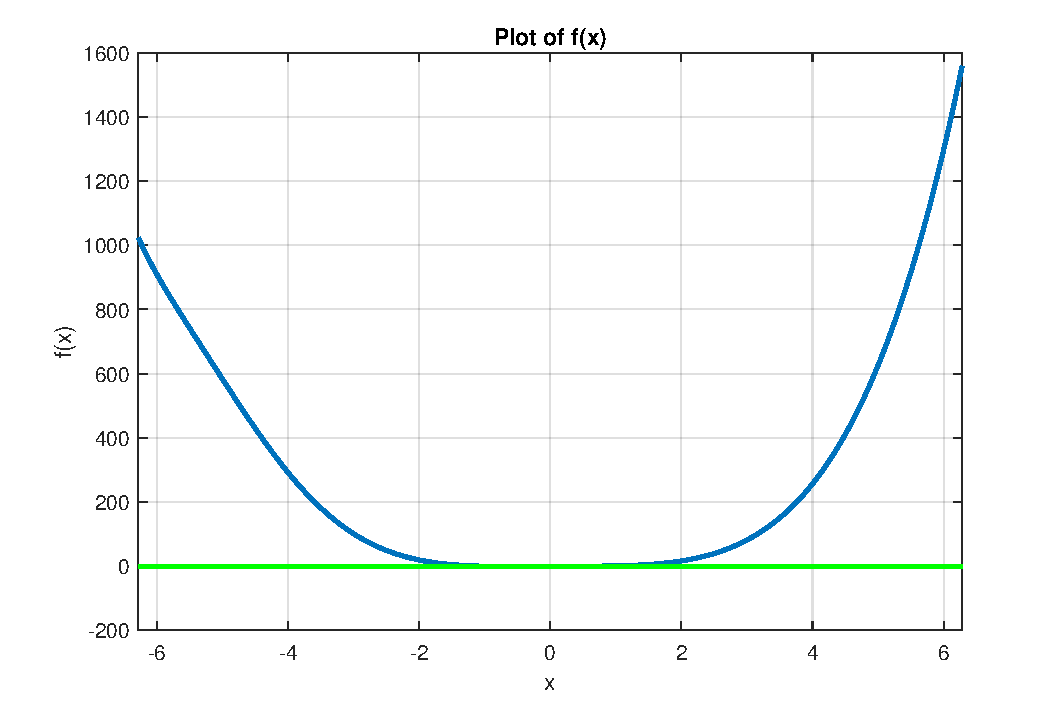
\includegraphics[scale=0.5]{images/Q1a_i.pdf}
			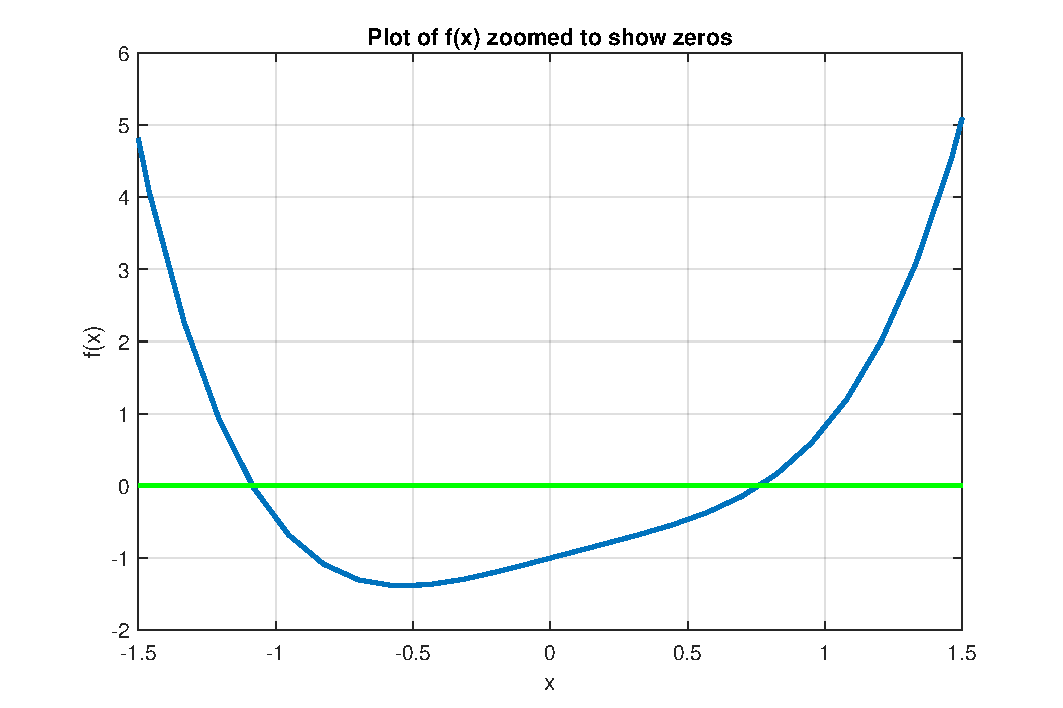
\includegraphics[scale=0.5]{images/Q1a_i_zoomed.pdf}
		}
			The second zoomed in plot shows there are two zeros in the given 
			domain. The first zero can be bracketed by the interval 
			$[-1.5,-1]$ as 
			$f(-1.5)=4.7455$ and $f(-1)=-0.4687$ so since the function is 
			continuous and there is a change of sign this bracket must 
			contain 
			a zero. Like wise the second root can be bracketed by the 
			interval $[0.5,1]$ 
			as $f(0.5)=-0.4698$ and $f(1)=0.8012$.
			
			
		\item Setting $f(x) = \frac{x^{3}}{\sin(x)} - 1$.
			\lstinputlisting{../src/q1/Q1a_ii.m}
		\NoIndent{
			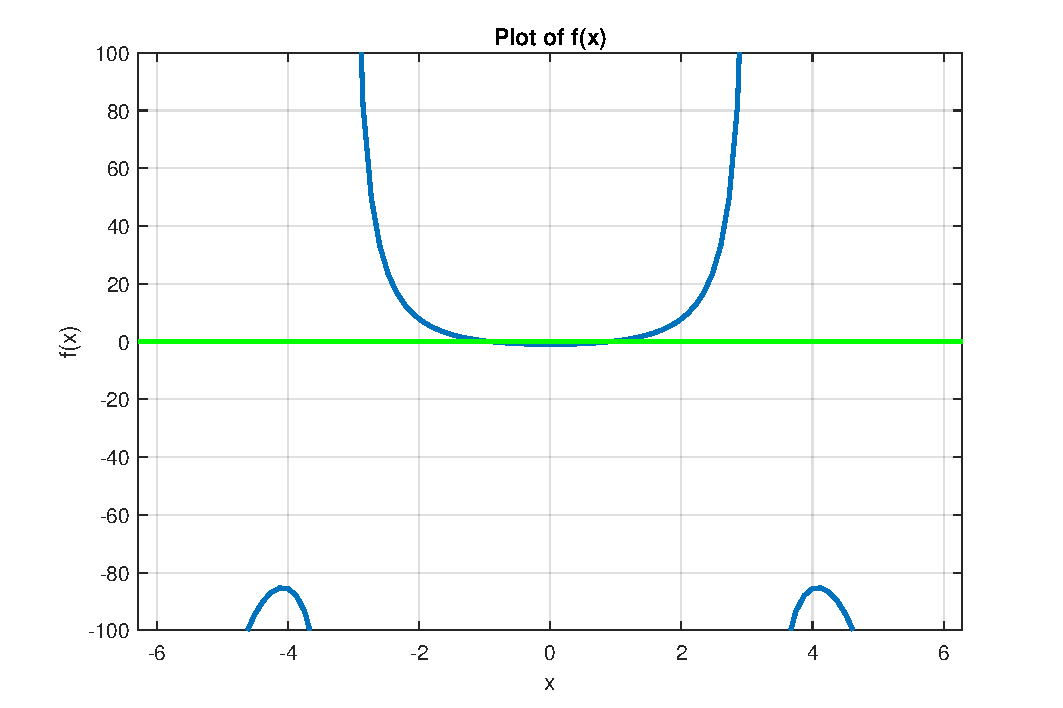
\includegraphics[scale=0.5]{images/Q1a_ii.pdf}
			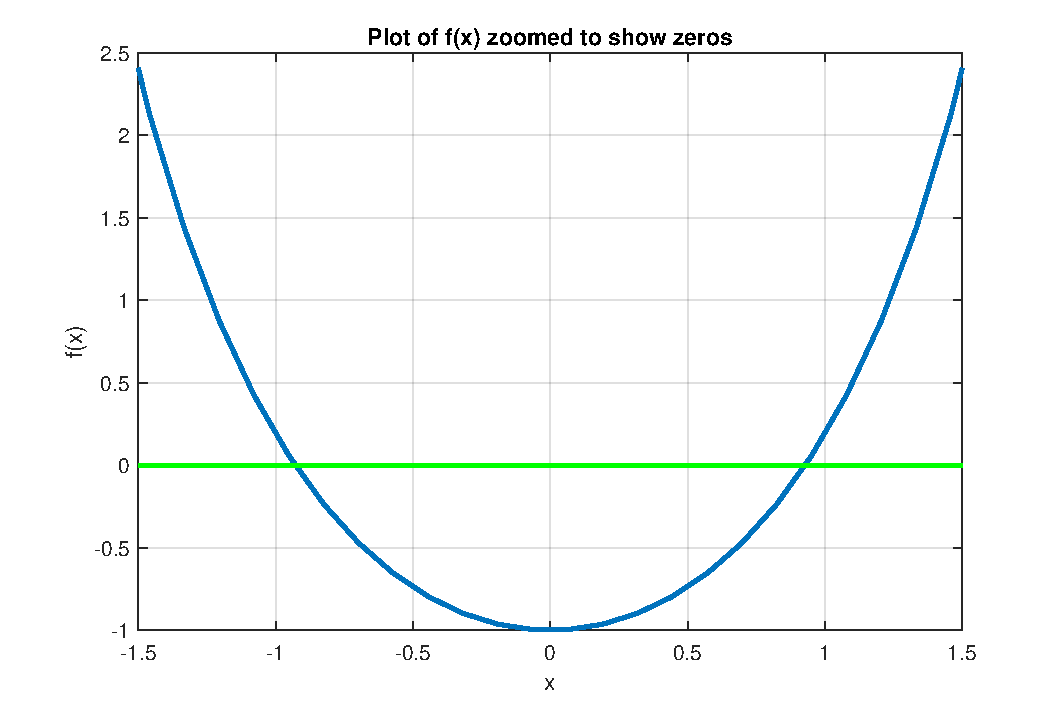
\includegraphics[scale=0.5]{images/Q1a_ii_zoomed.pdf}
		}
		The second plot show there are two roots. The first root can be 
		bracketed by the interval $[-1,-0.5]$ as $f(-1) = 0.1884$ 
		and 
		$f(-0.5)=-0.7393$ and $f(x)$ is continuous in this bracket. Likewise, 
		the second root can be bracketed by the interval $[0.5,1]$ as 
		$f(0.5)=-0.7393$ and 
		$f(1)=0.1884$.
		
		
		\item Rearranging $\cot(x) = \frac{25}{25x-1}$ gives $f(x) = \cot(x) 
		- \frac{25}{25x-1}$.
		\lstinputlisting{../src/q1/Q1a_iii.m}
		\begin{center}
			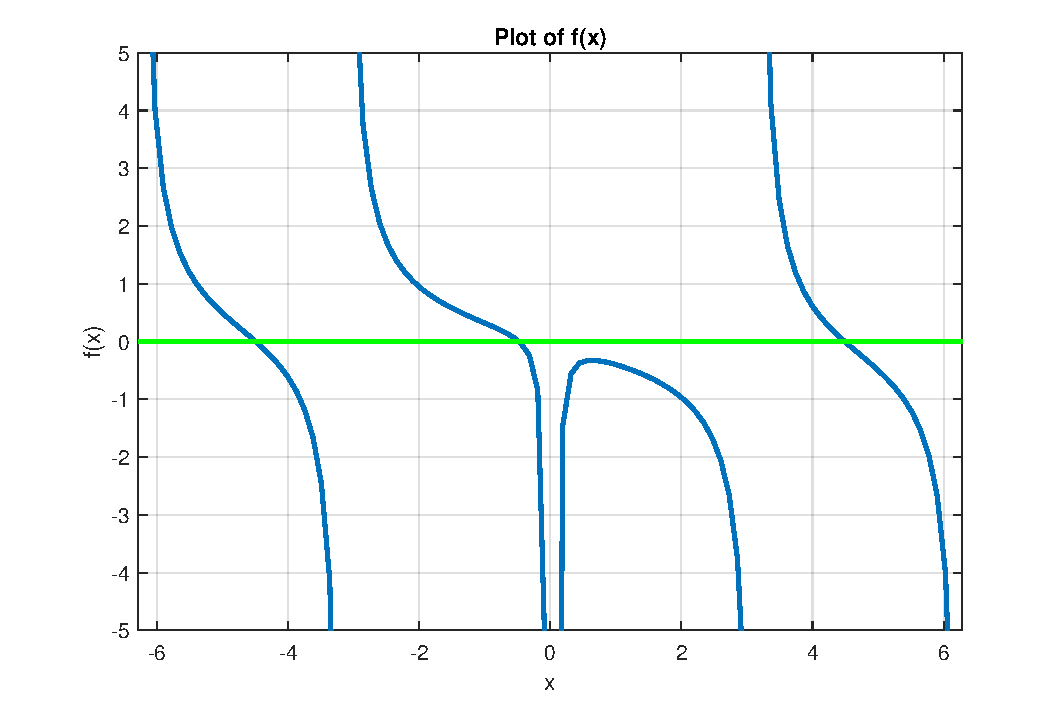
\includegraphics[scale=0.5]{images/Q1a_iii.pdf}
		\end{center}
		The plot shows that the equation has three solutions. The first can 
		be bracketed by the interval $[-5,-4]$ as $f(-5)=0.4942$ and 
		$f(-4)=-0.6162$. The 
		second solution can be bracketed by the interval $[-1,-0.1]$ as 
		$f(-1)=0.3194$ and 
		$f(-0.1)=-2.8238$. The third solution can be bracketed by the 
		interval $[4,5]$ as 
		$f(4)=0.6112$ and $f(5)=-0.4974$. $f(x)$ is continuous in each of the 
		bracketing intervals.
	
	
		\item Rearranging $4e^{-x^{2}/5} = cos(5x) + 2$ gives $f(x) = 
		4e^{-x^{2}/5} - cos(5x) - 2$.
		\lstinputlisting{../src/q1/Q1a_iv.m}
		\NoIndent{
		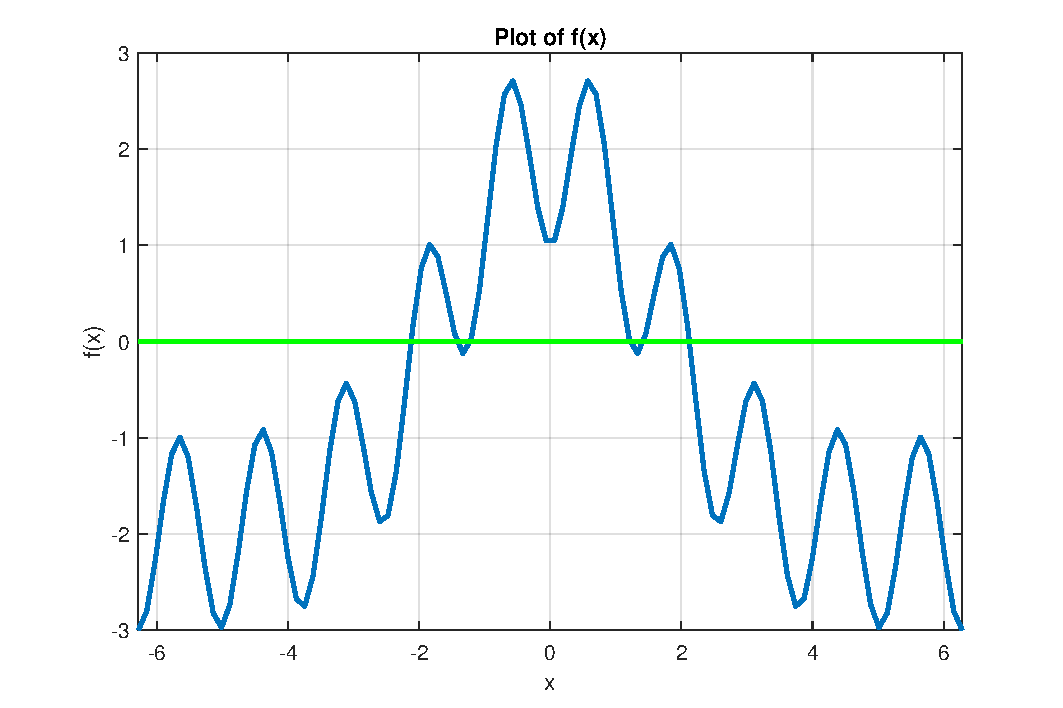
\includegraphics[scale=0.5]{images/Q1a_iv.pdf}
		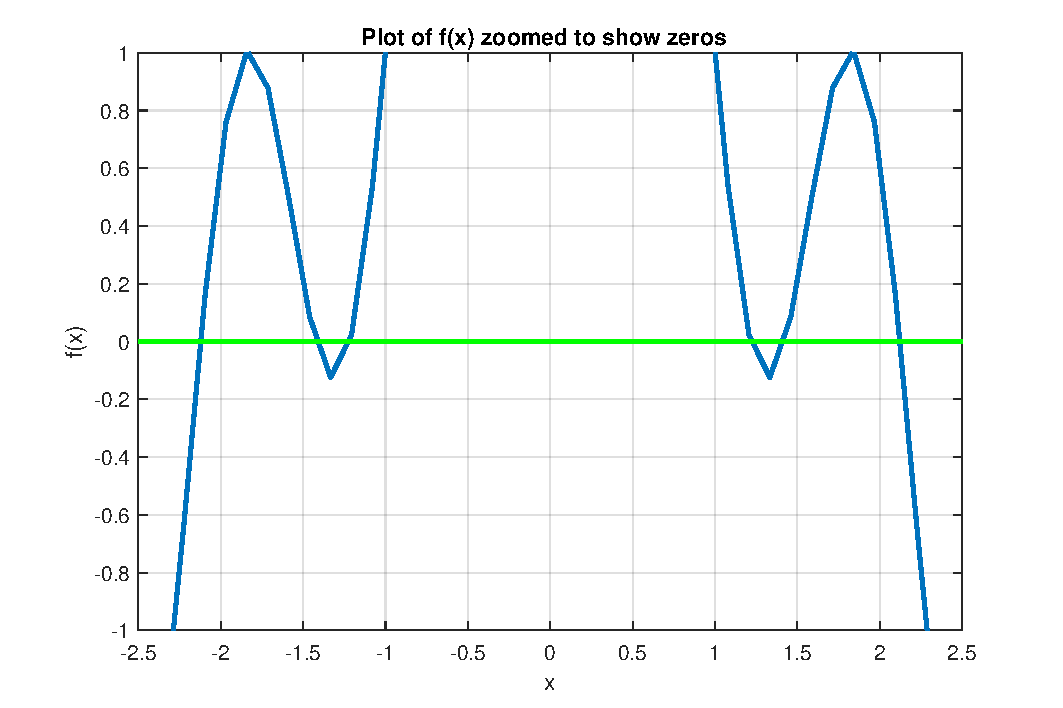
\includegraphics[scale=0.5]{images/Q1a_iv_zoomed.pdf}
		}
		The second plot shows that the equation has 6 solutions. The 
		bracketing intervals are shown in the table below.
		\begin{table}[!h]
			\centering
			\begin{tabular}{l|ll}
				$[a,b]$        & f(a)    & f(b)    \\ \hline
				$[-2.5,-2]$    & -1.8518 & 0.6364  \\
				$[-1.5,-1.25]$ & 0.2039  & -0.0730 \\
				$[-1.25,-1]$   & -0.0730 & 0.9913  \\
				$[1,1.25]$     & 0.9913  & -0.0730 \\
				$[1.25,1.5]$   & -0.0730 & 0.2039  \\
				$[2,2.5]$      & 0.6364  & -1.8518
			\end{tabular}
		\end{table}
	\end{enumerate}



	\item The bisection method is used by calling the the \verb*|bisectRoot| 
	function.
	\lstinputlisting[label=lst:bisect]{../src/q1/bisectRoot.m}
	
	
	\begin{enumerate}
		\item Solutions to $f(x) = x^{4} - e^{-x} \cos(x) = 0 \  \ 
		x\in[-2\pi,2\pi]$.
		\lstinputlisting{../src/q1/Q1b_i.m}
		Note the two different tolerances since one root is an order of 
		magnitude larger so requires one less decimal place of accuracy to be 
		accurate to 8 significant figures.
		\begin{table}[!h]
			\centering
			\begin{tabular}{l|ll}
				$[a,b]$     & Root       & \# Iterations \\ \hline
				$[-1.5,-1]$ & -1.0843597 & 23           \\
				$[0.5,1]$   & 0.76221107 & 26          
			\end{tabular}
		\end{table}
	
	
		\item Solutions to $f(x) = \frac{x^{3}}{\sin(x)} - 1 = 0 \  \ 
		x\in[-2\pi,2\pi]$.
		\lstinputlisting{../src/q1/Q1b_ii.m}
		\begin{table}[!h]
			\centering
			\begin{tabular}{l|ll}
				$[a,b]$     & Root        & \# Iterations \\ \hline
				$[-1,-0.5]$ & -0.92862631 & 26            \\
				$[0.5,1]$   & 0.92862631  & 26           
			\end{tabular}
		\end{table}
	
	
		\item Solutions to $f(x) = \cot(x)	- \frac{25}{25x-1} = 0 \  \ 
		x\in[-2\pi,2\pi]$.
		\lstinputlisting{../src/q1/Q1b_iii.m}
		\begin{table}[!h]
			\centering
			\begin{tabular}{l|ll}
				$[a,b]$     & Root        & \# Iterations \\ \hline
				$[-5,-4]$   & -4.4953722  & 24            \\
				$[-1,-0.1]$ & -0.47773376 & 27            \\
				$[4,5]$     & 4.4914097   & 24           
			\end{tabular}
		\end{table}
		
		
		\item Solutions to $f(x) = 4e^{-x^{2}/5} - cos(5x) - 2 = 0 \  \ 
		x\in[-2\pi,2\pi]$.
		\lstinputlisting{../src/q1/Q1b_iv.m}
		\begin{table}[!h]
			\centering
			\begin{tabular}{l|ll}
				$[a,b]$        & Root       & \# Iterations \\ \hline
				$[-2.5,-2]$    & -2.1222382 & 23            \\
				$[-1.5,-1.25]$ & -1.4255432 & 22            \\
				$[-1.25,-1]$   & -1.2145933 & 22            \\
				$[1,1.25]$     & 1.2145933  & 22            \\
				$[1.25,1.5]$   & 1.4255432  & 22            \\
				$[2,2.5]$      & 2.1222382  & 23           
			\end{tabular}
		\end{table}
	\end{enumerate}


	\item The iterative scheme we asked to implement is called Steffensen's 
	method. This is implemented in the \verb*|steffensenRoot| function.
	\lstinputlisting[label=lst:steph]{../src/q1/steffensenRoot.m}
	The following uses this function to find the root of $e^{-x} - x = 0$ and 
	calculate the convergence.
	\lstinputlisting{../src/q1/Q1c.m}
	After 5 iterations the root $x = 0.567143290410$ is accurate to 12 
	decimal places.
	\begin{center}
		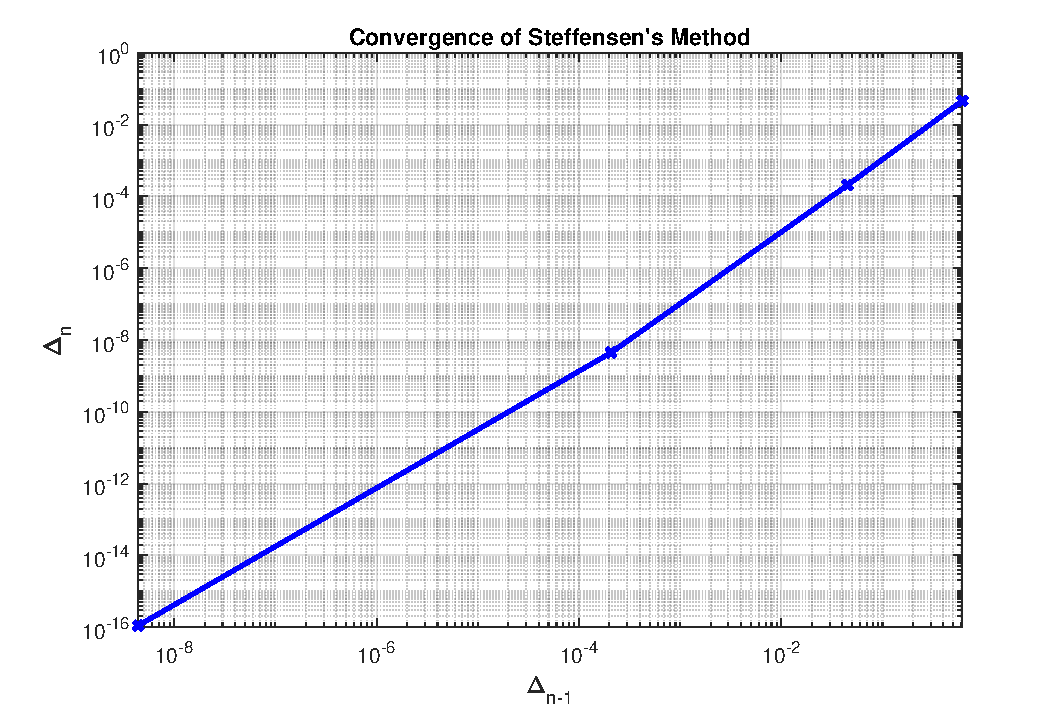
\includegraphics[scale=0.6]{images/Q1c.pdf}
	\end{center}
	The graph shows a straight which shows error $\propto \Delta_{n-1}^{q}$, 
	where q is the gradient of the line. Using the \verb*|MATLAB| function 
	\verb*|polyfit| the gradient of the 
	above graph as 1.8 which is close to 2 so Steffensen's method is second 
	order.
	
	
	\item The first step in creating a cobweb plot is to implement a fixed 
	point iteration scheme.
	\lstinputlisting{../src/q1/fixedPointRoot.m}
	\lstinputlisting{../src/q1/cobwebDiagram.m}
\end{enumerate}

\section{Numerical integration and differentiation}
\begin{enumerate}
	\item \begin{enumerate}
		\item The first expression is Simpson's 3/8 rule and the second is 
		Milne's rule.
		
		Simpson's 3/8 rule can be implemented as follows.
		\lstinputlisting{../src/q2/simpson38.m}
		And similarly Milne's rule can be implemented.
		\lstinputlisting{../src/q2/milne.m}
		However to use the composite version the integral must be broken down 
		into smaller intervals. For example breaking the integral into $n$ 
		intervals gives $\int_{a}^{b}f(x)dx = \int_{a}^{x_{1}}f(x)dx + 
		\int_{x_{1}}^{x_{2}}f(x)dx + \cdots + \int_{x_{n-1}}^{b}f(x)dx$ 
		where 
		$x_{i} = a + i \cdot \frac{b - a}{n}$. Then each of these smaller 
		integrals can be calculated using either of the methods. The 
		\verb*|compositeQuad| function breaks down the integral into smaller 
		intervals before using a Newton-Coutes method of choice to 
		approximate the integral.
		\lstinputlisting{../src/q2/compositeQuad.m}
		For an example both methods can be used to evaluate $\int_{0}^{5} 
		e^{x} - x dx$ to 6 decimal places as follows.
		\lstinputlisting{../src/q2/Q2ai_example.m}
		Both give the answer to the example as $134.913159$.
		
		
		\item Find order and accuracy
	\end{enumerate}

	
	\item \begin{enumerate}
		\item To find the order of the rounding and truncation error the 
		absolute error is plotted against $h$.
		\begin{center}
			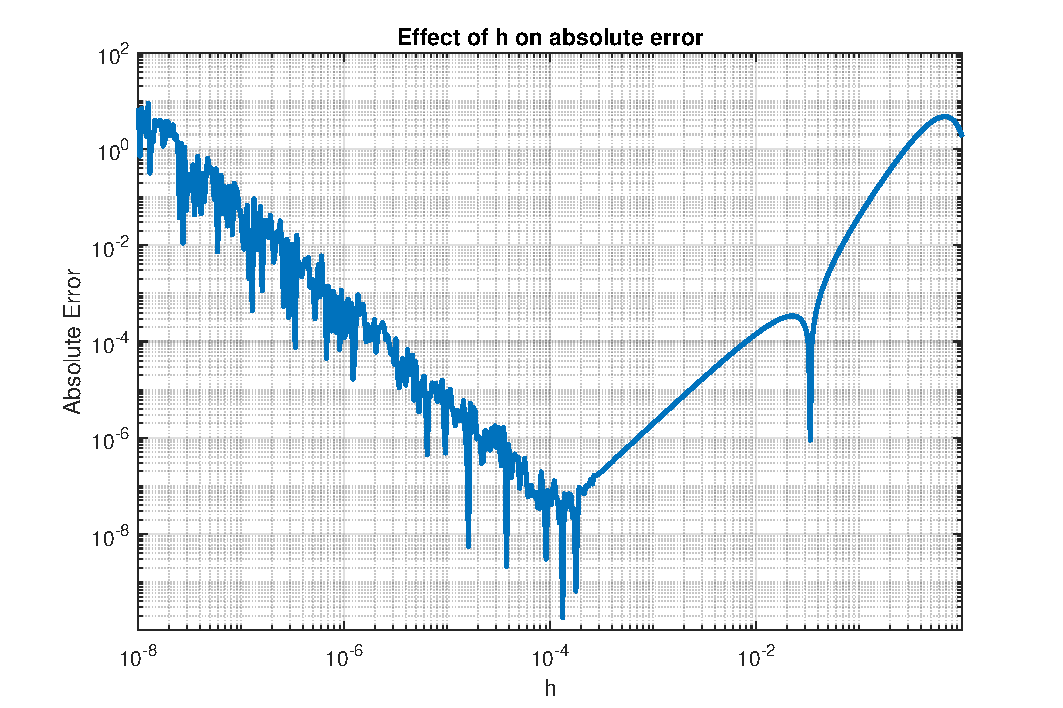
\includegraphics[scale=0.7]{images/Q2bi.pdf}
			\captionof{figure}{Plot generated by \autoref{lst:q2bi}}
		\end{center}
		The gradient of the two sections of the graph shows the order of the 
		rounding and truncation error. The rounding error is shown by the 
		jagged first half which has a gradient of -2 which shows the order of 
		the rounding error is $\mathcal{O}(h^{-2})$. The second half of the 
		graph shows the truncation error. This has a gradient of 2 which 
		shows the truncation error is $\mathcal{O}(h^{2})$.
		
		\item The error is comprised of the truncation and rounding error. To 
		find the truncation error of 
		\begin{equation}
			f''(x) \approx \frac{2f(x)-5f(x+h)+4f(x+2h)-f(x+3h)}{h^{2}},
			\label{eq:f''}
		\end{equation}
		consider the following taylor expansions
		\begin{equation}
			f(x + h) = f(x) + hf'(x) + \frac{h^{2}}{2}f''(x) + 
			\frac{h^{3}}{6}f^{(3)}(x) + \frac{h^{4}}{24}f^{(4)}(x) + \cdots,
			\label{eq:t1}
		\end{equation}
		\begin{equation}
			f(x + 2h) = f(x) + 2hf'(x) + \frac{4h^{2}}{2}f''(x) + 
			\frac{8h^{3}}{6}f^{(3)}(x) + \frac{16h^{4}}{24}f^{(4)}(x) + 
			\cdots,
			\label{eq:t2}
		\end{equation}
		\begin{equation}
			f(x + 3h) = f(x) + 3hf'(x) + \frac{9h^{2}}{2}f''(x) + 
			\frac{27h^{3}}{6}f^{(3)}(x) + \frac{81h^{4}}{24}f^{(4)}(x) + 
			\cdots.
			\label{eq:t3}
		\end{equation}
		Substituting \eqref{eq:t1}, \eqref{eq:t2}, \eqref{eq:t3} into 
		\eqref{eq:f''} gives
		\begin{align}
			f''(x) &\approx \frac{h^{2}f''(x) + 
			\frac{-11}{12}h^{4}f^{(4)}(x) + \mathcal{O}(h^{5})}{h^{2}}\\
			&= f''(x) - \frac{11}{12}h^{2}f^{(4)}(x) + 
			\mathcal{O}(h^{3}),
		\end{align}
		so the truncation error is $\frac{11}{12}h^{2}f^{(4)}(x) + 
		\mathcal{O}(h^{3})$.
		
		To find the rounding error assume $h$ is small and can be stored 
		exactly. So the rounding error in storing $f(x)$, $f(x+h)$, $f(x+2h)$ 
		and $f(x+3h)$ is $|f(x)|\epsilon$, where $\epsilon$ is the floating 
		point relative accuracy, $2\times 10^{-16}$. This means the total 
		rounding error is $\frac{12|f(x)|\epsilon}{h^{2}}$. So the total 
		error is given by
		\begin{equation}
			\text{error} \approx \frac{11}{12}h^{2}f^{(4)}(x) + 
			\frac{12|f(x)|\epsilon}{h^{2}}.
		\end{equation}
		We want to minimise the error so
		\begin{equation}
			\frac{d}{dt}\text{error} \approx \frac{22}{12}hf^{(4)}(x) - 
			\frac{24|f(x)|\epsilon}{h^{3}}=0.
		\end{equation}
		Approximating $f(x)\approx f^{(4)}(x)$ gives
		\begin{equation}
			\frac{22}{12}h - 
			\frac{24\epsilon}{h^{3}}=0,
		\end{equation}
		so the h which minimises the error is
		\begin{equation}
			h = \sqrt[4]{\frac{144}{11}\epsilon}.
		\end{equation}
		\begin{center}
			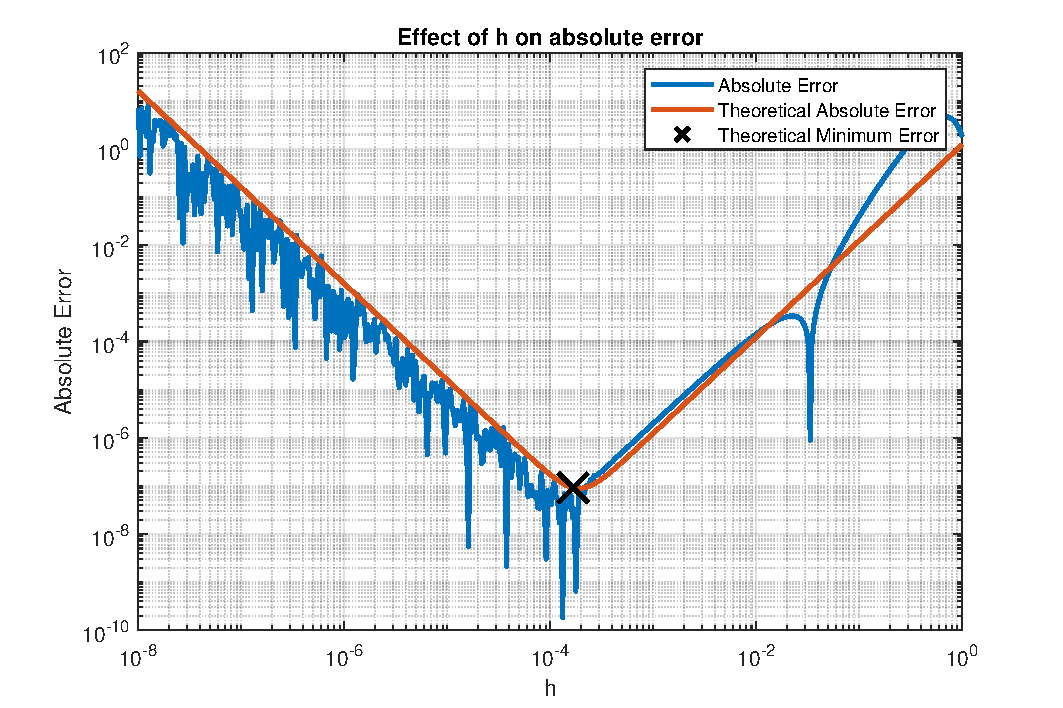
\includegraphics[scale=0.7]{images/Q2bii.pdf}
			\captionof{figure}{Plot produced using \autoref{lst:q2bii}}
		\end{center}
		The algebraic expression has the same gradient however it is offset. 
		This is because it assumes that $h$ can be stored exactly and because 
		it assumes $f(x)\approx f^{(4)}(x)$. However the value of h that 
		minimises error lines up correctly.
	\end{enumerate}
\end{enumerate}

\section{Numerical solution of ODEs}
\begin{enumerate}
	\item \lstinputlisting{../src/q3/rhsProjectile.m}
	
	
	\item\begin{enumerate}
		\item Forward Euler
		\lstinputlisting{../src/q3/forwardEulerProjectile.m}
		\item 4th-order Runge-Kutta
		\lstinputlisting{../src/q3/rk4Projectile.m}
		\item \verb*|ode45|
		\lstinputlisting{../src/q3/ode45projectile.m}
	\end{enumerate}


	\item Solving the ODE using the three different solvers gives the 
	following trajectories.
	\begin{center}
		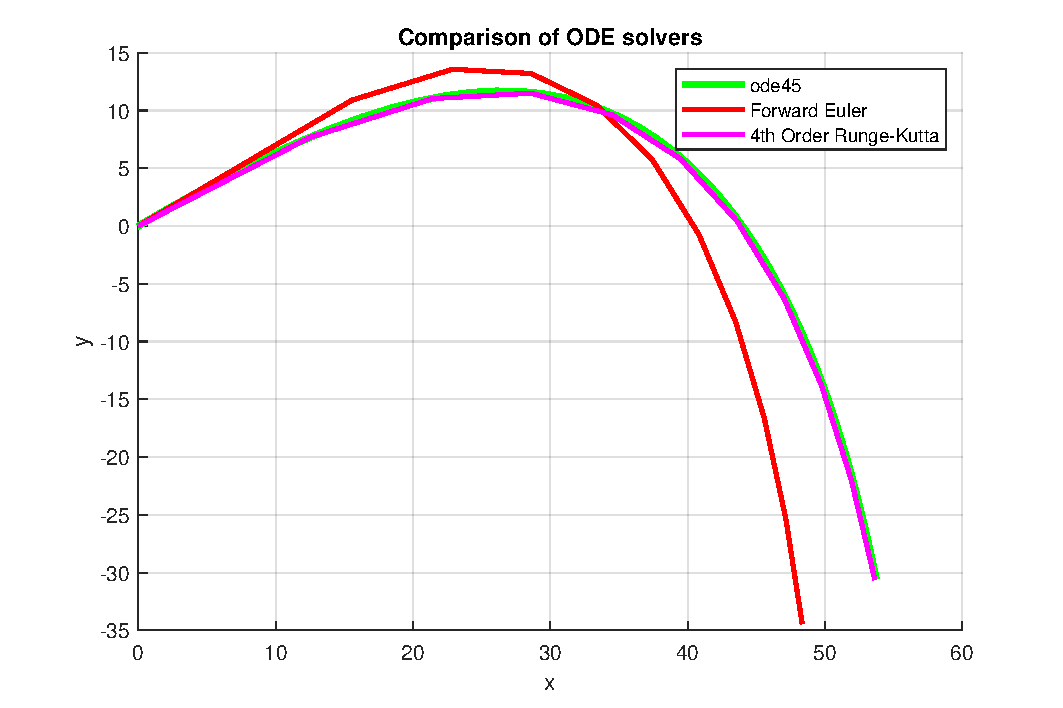
\includegraphics[scale=0.7]{images/Q3c.pdf}
		\captionof{figure}{Plot produced using \autoref{lst:q3c}}
	\end{center}

	
	\item Error compared to \verb*|ode45|.
	\begin{center}
		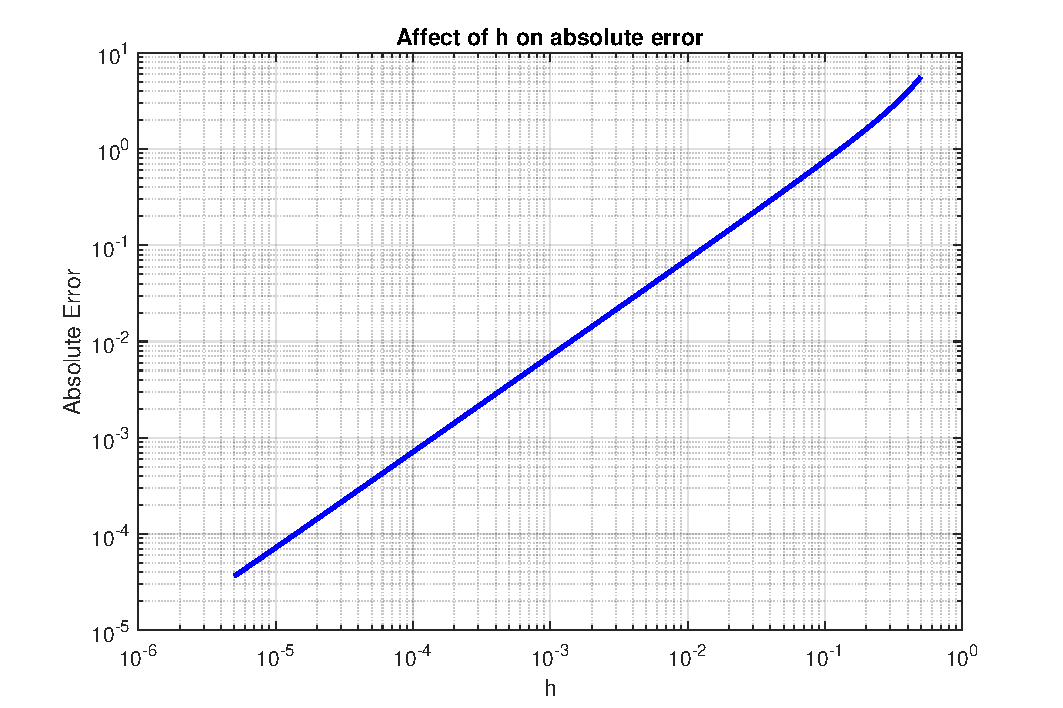
\includegraphics[scale=0.7]{images/Q3d.pdf}
		\captionof{figure}{Generated using \autoref{lst:q3d}}
	\end{center}
	The order of global truncation error can be given by the gradient in the 
	limit as $h \xrightarrow{} 0$. In this case the gradient is 1 so the 
	global truncation error is $\order(h)$.
	
	\item To find when the projectile crosses the x-axis first an event 
	function is created.
	\lstinputlisting{../src/q3/xaxisEvent.m}
	Then solve the ODE with the added event function.
	\lstinputlisting{../src/q3/Q3e.m}
	This gives that the projectile first passes through the x-axis when 
	$t=3.038777368718$
	
	
	\item An equivalent formulation to this problem is to consider the angles 
	$\theta_{0}$ required so that when a particle is fired from $(-40,0)$ it 
	lands through the origin $(0,0)$. This can be visualized by plotting the 
	landing $x$ coordinate against $\theta_{0}$ as shown in 
	\autoref{fg:landing}.
	\begin{center}
		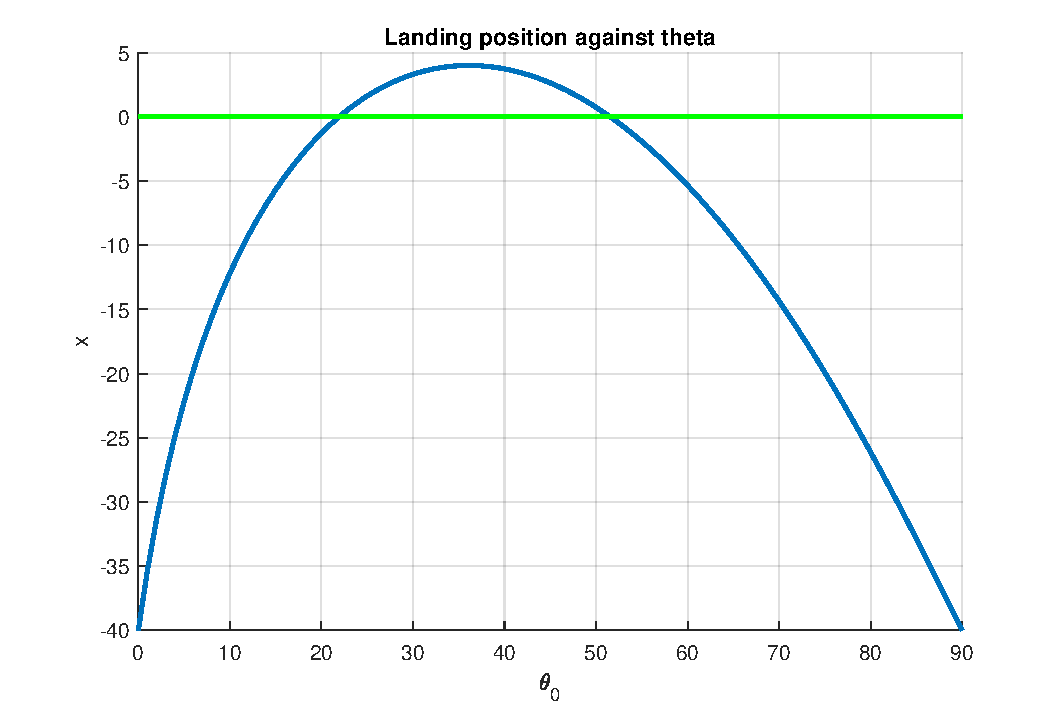
\includegraphics[scale=0.7]{images/Q3f.pdf}
		\captionof{figure}{Generated using \autoref{lst:q3f}}
		\label{fg:landing}
	\end{center}
	This shows the problem can be reduced to a root finding problem. This can 
	be done using the bisection method already implemented in 
	\autoref{lst:bisect} or Stephen's method implemented in 
	\autoref{lst:steph}. The two values of $\theta_{0}$ can be bracketed by 
	the 
	intervals $[20,25]$ and $[50,55]$. First a function, $x(\theta_{0})$, 
	that 
	returns just the 
	landing 
	position given a $\theta_{0}$ needs to be created.
	\lstinputlisting{../src/q3/landingPosition.m}
	Then using the bisection method the roots of $x(\theta_{0}) = 0$ can be 
	found.
	\lstinputlisting{../src/q3/Q3f_theta_solution.m}
	This gives $\theta_{0} = 21.9185709$ or $\theta_{0} = 51.567361$.
\end{enumerate}

\newpage
\begin{appendices}
	\section{Additional Code for Question 1}
	\section{Additional Code for Question 2}
	\lstinputlisting[label=lst:q2bi]{../src/q2/Q2bi.m}
	\lstinputlisting[label=lst:q2bii]{../src/q2/Q2bii.m}
	\section{Additional Code for Question 3}
	\lstinputlisting[label=lst:q3c]{../src/q3/q3c.m}
	\lstinputlisting[label=lst:q3d]{../src/q3/q3d.m}
	\lstinputlisting[label=lst:q3f]{../src/q3/Q3f.m}
\end{appendices}

\end{document}
